\renewcommand\chapterillustration{abertura-superficie}%Photo by Hoach Le Dinh on Unsplash, https://unsplash.com/photos/c8TWWQ5ZnUw?utm_source=unsplash&utm_medium=referral&utm_content=creditCopyText 
\renewcommand\chapterwhat{A partir de situações do cotidiano, mesmo que uma superfície não seja plana, entender o conceito de área de modo que possa diferenciá-lo de outras grandezas, e identificar suas propriedades. Estabelecer métodos de medição da grandeza “área” e interpretá-los em contextos reais. }
\renewcommand\chapterbecause{É fundamental saber identificar e determinar áreas de figuras planas ou espaciais visto que, em atividades cotidianas, temos a necessidade de realizar medições de áreas para resolver problemas. Para poder explorar os problemas práticos, é fundamental conhecer o conceito de área de uma figura, como um tópico que permite compreender as expressões que trabalham os elementos determinantes do conceito de área, e os procedimentos que as aplicações práticas demandam.}
\chapter{Áreas de superfície}
\label{est1-chap}

\mbox{}\thispagestyle{empty}\clearpage

\thispagestyle{empty}

\begin{center}
Projeto: LIVRO ABERTO DE MATEMÁTICA

\noindent \begin{tabular}{lcccr}

\includegraphics[scale=.15]{impa}& \quad\quad& 
\includegraphics[width=3cm]{logo} & \quad\quad& 
\includegraphics[scale=.24]{obmep} 
\end{tabular}
\end{center}

\vspace*{.3cm}

Cadastre-se como colaborador no site do projeto: \url{umlivroaberto.org}

Versão digital do capítulo:

\url{https://www.umlivroaberto.org/BookCloud/Volume_1/master/view/PE103.html}

% \begin{center}
%   \includegraphics[width=2cm]{canvas}
% \end{center}

\begin{tabular}{p{.15\textwidth}p{.7\textwidth}}
Título: & Áreas de Superfícies\\
\\
Ano/ Versão: & 2020 / versão 0.2 de 16 de outubro de 2020\\
\\
Editora & Instituto Nacional de Matem\'atica Pura e Aplicada (IMPA-OS)\\
\\
Realização:& Olimp\'iada Brasileira de Matem\'atica das Escolas P\'ublicas (OBMEP)\\
\\
Produção:& Associação Livro Aberto\\
\\
Coordenação: & Fabio Simas, \\
             & Augusto Teixeira (livroaberto@impa.br)\\
\\
  Autores: & Flávia Landim (coordenadora da equipe - UFRJ),\\
        & José Ezequiel Soto Sanches,\\
        & Nei Rocha (UFRJ),\\
             & Vanessa Matos (SEduc Angras dos Reis e Mesquita).\\
             & Letícia Rangel (Colégio de Aplicação da UFRJ)\\
\\
Revisão: &  Cydara Ripoll  \\
		 &  Letícia Rangel
\\
Design: & Andreza Moreira (Tangentes Design) \\
\\
  Ilustrações: & --- \\ 
\\
Gráficos: & ---\\
\\
  Capa: & Foto de Chuttersnap no Unsplash \\
        & https://unsplash.com/photos/8I423fRMwjM \\

\end{tabular}



\begin{figure}[b]
\begin{minipage}[l]{5cm}
\centering

{\large Licença:}

  
\includegraphics[width=3.5cm]{cc-by-nc-sa}
\end{minipage}\hfill
\begin{minipage}[c]{5cm}
\centering
{\large Desenvolvido por}


\includegraphics[width=2.5cm]{logo-associacao.jpg}
\end{minipage}
\begin{minipage}[r]{5cm}
\centering

{\large Patrocínio:}
  \vspace{1em}
  
\includegraphics[width=3.5cm]{itau}
\end{minipage}
\end{figure}

\mainmatter

\explore{O que é área?}

Saber resolver problemas utilizando o conceito de área, nos mais diferentes contextos, dentro da Matemática ou com outras áreas do conhecimento é a objetivo deste capítulo. Contextos significativos, não somente no contexto escolar, mas também em questões ligadas a comunidade e ao mundo do trabalho. Ao final desta unidade espera-se que você, estudante, seja capaz de, por exemplo,  calcular a quantidade de tinta necessária para pintar uma casa, não desperdiçar tecido para fabricar uma peça de roupa, determinar a área de terrenos, calcular a quantidade de lajotas para cobrir pisos e paredes, determinar a área de faces de objetos, entre tantos outros problemas ligados ao conceito de área.

\begin{task}{O Parque Estadual do Turvo}

\begin{multicols}{2}

O Parque Estadual do Turvo, criado em de 11 de março de 1947, como Reserva Florestal, foi uma das primeiras unidades de conservação instituídas no Rio Grande do Sul em 1954, sendo a maior área protegida de proteção integral do Estado.

\begin{figure}[H]
\centering

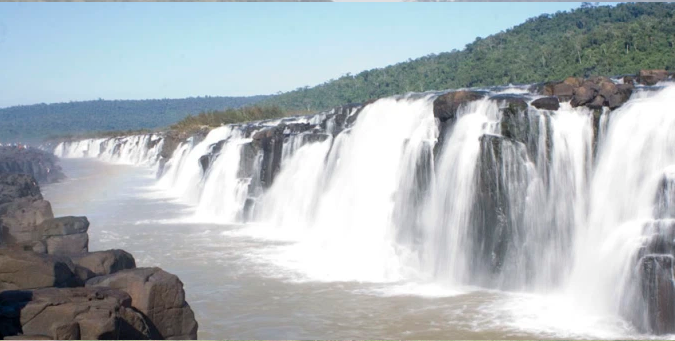
\includegraphics[width=200bp]{superficie1}

\caption{Salto do Yucumã, Parque Estadual do Turvo. Foto: D. Meller}
\end{figure}

\end{multicols}

É o último refúgio para animais como a onça-pintada, a anta e o gavião-real (harpia) no Rio Grande do Sul. Por tais atributos é considerado por muitos ambientalistas como a área mais importante para conservação da fauna gaúcha ameaçada de extinção. O principal atrativo turístico do parque é o Salto do Yucumã, a maior queda d’água longitudinal do mundo, com 1800 metros de extensão.

Situa-se no município de Derrubadas, no extremo Noroeste do Rio Grande do Sul, Brasil. Através do Rio Uruguai faz fronteira com a província argentina de Misiones e divisa com o estado brasileiro de Santa Catarina (\url{https://parquedoturvo.wordpress.com}).

\begin{figure}[H]
\centering

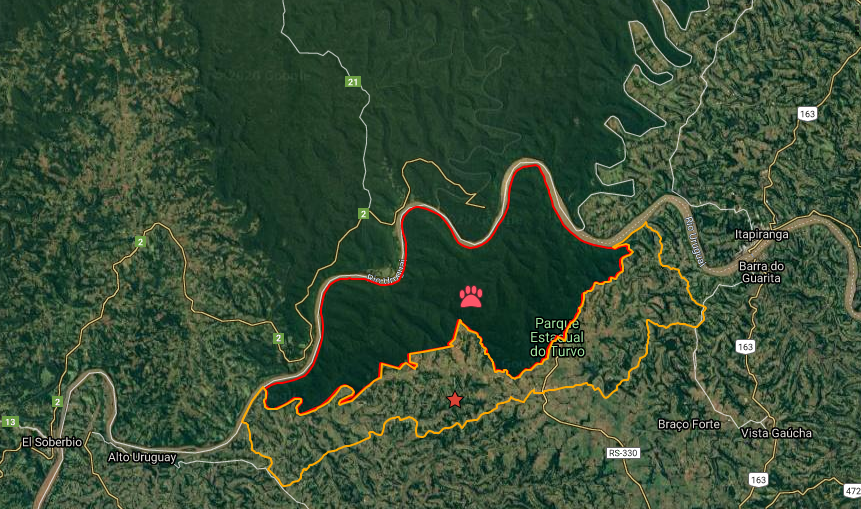
\includegraphics[width=300bp]{superficie2}

\end{figure}

\begin{enumerate}
  \item É possível calcular a área e o perímetro do parque? Discuta com seu grupo e descreva um método para obter a área e o perímetro da região anterior.
  \item Com o auxílio de \textit{Google My Maps}, calcule a área e o perímetro aproximado do Parque Estadual do Turvo.
\end{enumerate}
\end{task}

\begin{task}{Outras experiências}
Uma folha retangular de papel foi cortada de um vértice ao vértice oposto, formando dois pedaços. Qual pedaço te perímetro maior?
\begin{figure}[H]
\centering

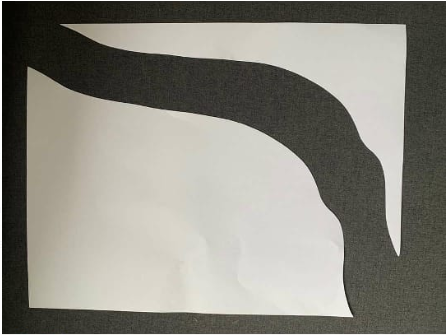
\includegraphics[width=200bp]{superficie3}

\end{figure}
\end{task}

\begin{task}{Podencial híbrido de uma planta}
(Atividade adaptada de \href{http://www.phschool.com/science/biology_place/labbench/lab9/calcsurf.html}{Pearson Prentice Hall})

\begin{wrapfigure}{r}{.5\textwidth}
\centering
  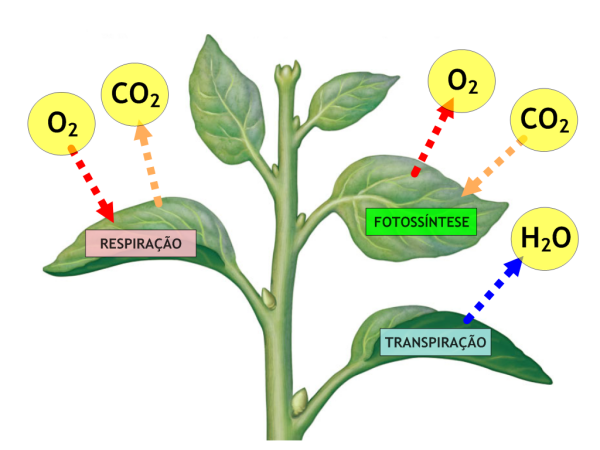
\includegraphics[width=200bp]{superficie4.png}
  \caption{Fonte: \href{https://www.estudokids.com.br/respiracao-e-transpiracao-dos-vegetais/)}{Estudo Kids}}
\end{wrapfigure}  
A respiração é essencial para a sobrevivência de todos os animais e também dos vegetais. Quando os seres vivos respiram, o oxigênio que está presente no ar é inspirado e o gás carbônico é expirado. Todos os seres vivos passam por esse processo, inclusive as plantas. A transpiração dos vegetais é um processo que ocorre quando a planta absorve água em excesso. 

Assim como na respiração, a principal parte do vegetal que é responsável por realizar a transpiração é a folha. Com o intenso calor e tempo seco de alguns lugares, os vegetais passaram a evoluir obtendo, desta forma, mecanismos reguladores quanto à absorção, retenção e perda de água. O excesso de água desses vegetais é liberado pelas folhas para o meio ambiente através de pequenas gotinhas de água que se transformam em vapor. Quando as temperaturas estão muito elevadas em certo período do dia, a planta fecha seus estômatos para não perder muita água para o meio ambiente e consequentemente ficar desidratada.

É importante saber que a quantidade de folhas e a superfície foliar são fatores determinantes para a maior ou menor taxa de transpiração, isso acontece devido às células estomáticas. A taxa de transpiração é medida como a quantidade de água perdida por m$^2$ e por minuto. Para chegar à taxa de transpiração, portanto, você deve calcular a área de superfície foliar de cada planta: 

\begin{figure}[H]
\centering

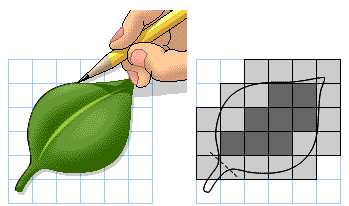
\includegraphics[width=200bp]{superficie5}

\end{figure}

\begin{itemize}
  \item Coloque as folhas a serem medidas em uma grade de $1$cm e trace seus contornos.
  \item Conte o número de centímetros quadrados. Estime a área dos quadrados parciais (conte um quadrado parcial se estiver pelo menos metade coberto pela folha; não conte quadrados parciais com menos do que meio coberto).
  \item Não inclua a área da haste (pecíolo) em seus cálculos.
\end{itemize}

\begin{enumerate}
  \item Consiga algumas folhas de tamanhos diferentes e calcule a sua área.
  \item Como a água evapora através dos muitos estômatos (são estruturas da epiderme da planta localizadas nas folhas e responsáveis pelas trocas gasosas e pela transpiração) na superfície da folha, a taxa de transpiração está diretamente relacionada à área da superfície. O que significa isso?
\end{enumerate}
\end{task}
\clearpage
\begin{knowledge}
O cálculo da área de sua superfície ocorre de uma maneira especial. Observe a figura a seguir, ela representa a superfície de uma região plana irregular: 

\begin{figure}[H]
\centering

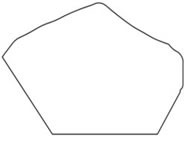
\includegraphics[width=150bp]{superficie6}

Figura A
\end{figure}

Para calcularmos a sua área uma opção é transpor a figura sobre um papel quadriculado, da seguinte forma: 

\begin{figure}[H]
\centering

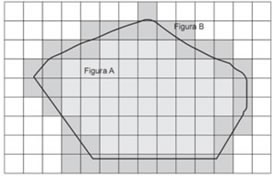
\includegraphics[width=175bp]{superficie7}

Figura B
\end{figure}

Realizada essa ação, é preciso contar o número de quadrados inteiros que preenchem o interior da figura. A área por falta da figura é de $43$ quadrados (figura A).

Observe que se, contar o número de quadrados inteiros que cobrem toda a figura, a área por excesso da região é de $80$ quadrados (figura B). 

Para determinarmos a área aproximada da figura, que está entre $43$ e $80$, utilizamos uma média aritmética da quantidade de quadriculados encontrados: 
\begin{equation*}
A=\frac{43+90}{2}=61{,}5.
\end{equation*}

A unidade de área utilizada será a da figura no tamanho original. Nesse caso, a área da figura dada se encontra em m$^2$, então, cada quadriculado representa $1$m$^2$. Portanto, a área da região irregular é de aproximadamente $61{,}5$m$^2$.

Fonte: \href{https://brasilescola.uol.com.br/matematica/calculo-de-areas-especiais.htm}{Brasil Escola}
\end{knowledge}

\begin{task}{Poluição por derramamento de petróleo}
(Atividade adaptada de \href{https://www.tecnologiae.com.br/poluicao-derramamento-petroleo-quais-consequencias/}{Tecnologia É})

Nosso planeta, a Terra, tem grandes reservas de petróleo e gás presas nas profundezas de sua superfície. Ocasionalmente, essas reservas desenvolvem rachaduras e parte do petróleo ou gás vaza. Nos últimos anos, a questão dos derramamentos de óleo e seus efeitos assumiu grande importância. Isso ocorre porque quando ocorre um derramamento de óleo há uma infinidade de problemas para o ambiente e para nós. Como derramamento de óleo, ele flutua na água e impede a passagem da luz solar. A substância brilhante que você vê, por vezes, na camada superior da água não é nada, mas é petróleo que torna difícil para as plantas e animais marinhos para sobreviverem. Limpar o derramamento de óleo não é tarefa fácil. Vários fatores precisam ser considerados antes de realizar as operações. Alguns deles sendo quantidade de óleo derramado, temperatura da água, tipo de praias e muito mais.

\begin{figure}[H]
\centering

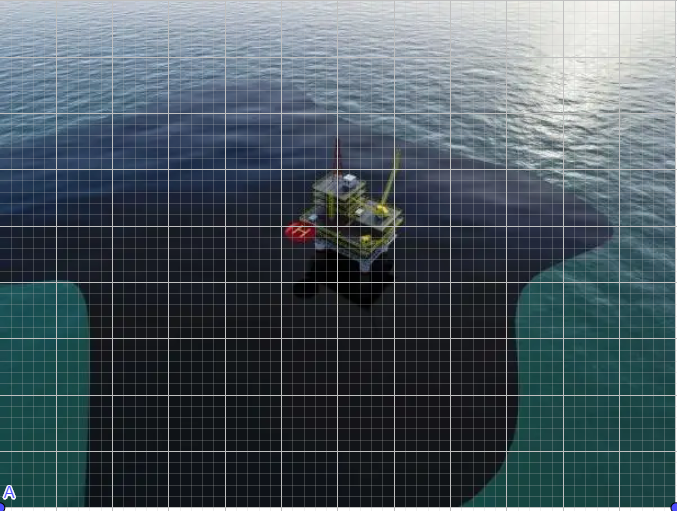
\includegraphics[width=325bp]{superficie8}


\caption{Foto: Times Now}
\end{figure}

\begin{enumerate}
  \item Calcule a área aproximada da mancha apresentada na foto acima
  \item Utilizando a escala do mapa, determine a área em km$^2$.
\end{enumerate}

\end{task}

\arrange{Conceituando área}

Para \textit{medir} uma grandeza devemos compará-la com uma outra de mesma espécie tomando-a como unidade. Assim, quando vamos medir uma porção do plano ocupada por uma figura, esta medida é a sua área.

\begin{quote}
Para encontrar a área de uma figura F, devemos comparar sua superfície (a porção do plano que ele ocupa) com a de uma outra figura tomada como unidade. O resultado dessa comparação será um número que deverá exprimir quantas vezes a figura F contém a unidade de área 
\flushright

(Lima, 2013, p. 92)
\end{quote}

A área de uma figura exprime quantas vezes essa figura contém uma \textit{unidade de área}. Observe a figura a seguir. Consideramos a unidade de área como cada triângulo.
\begin{multicols}{2}
\begin{figure}[H]
\centering

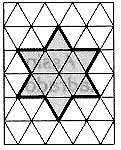
\includegraphics[width=100bp]{superficie9}
\end{figure}
\columnbreak

\null\vfill
\begin{figure}[H]
\centering

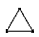
\includegraphics[width=25bp]{superficie10}
$1$ unidade de área

\medskip

Área de figura: 12 unidades de área
\end{figure}
\vfill\null
\end{multicols}

Em geral, adotamos como \textit{unidade de área} o quadrado cujo lado mede uma unidade de comprimento. Sendo assim, para cada unidade de comprimento existe uma unidade de área correspondente.

\begin{figure}[H]
\centering

\begin{tikzpicture}
\draw[fill=\currentcolor!80] (0,0) rectangle (1,1);
\draw [->] (0.5,0.5) -- (2.5,0.5) node [right] {$1$ unidade de área};
\node [below] at (.5,0) {$1$ unidade de comprimento};
\draw [very thick] (0,0) -- (1,0);
\end{tikzpicture}
\end{figure}

Assim, por exemplo, ao considerarmos um quadrado de lado $1$cm, a unidade de área será chamada de \textit{centímetro quadrado} (cm$^2$). Logo,



\begin{figure}[H]
\centering

\begin{tikzpicture}
\tikzstyle{quad}=[minimum width=1cm, minimum height=1cm, draw, node distance=1cm];

\node [fill=\currentcolor!80, quad] (a) {\small$1$cm$^2$};

\begin{scope}[xshift=4cm]
\node [fill=\currentcolor!80, quad] (a) {};
\node (b) [right of=a, quad] {};
\node (c) [below of=b, quad] {};
\node (d) [above of=b, quad] {};
\node (e) [right of=b, quad] {};

\node [below of=c] {Área da figura = $4$cm$^2$};
\end{scope}
\end{tikzpicture}
\end{figure}

Mas como poderemos comparar a superfície de uma figura qualquer com a unidade de área? Para figuras com formatos mais irregulares poderemos determinar a sua área por aproximações. Quanto mais preciso forem nossos métodos, melhor será a nossa aproximação.

\explore{área de figuras planas}

\begin{task}{a reforma da sala}

Marcelo pretende investir na reforma da sala de seu apartamento. Vai trocar o pixo, colocar gesso no teto, criar um painel de gesso e pintar. Para isso está pesquisando os materiais necessários.

\begin{table}[H]
\centering
\setlength\tabulinesep{3.5pt}
\setlength\tabcolsep{3pt}
\begin{tabu} to \textwidth{|l|ll|}
\hline
Piso laminado & Régua: $8\text{mm}\times187\text{mm}\times 1350$mm & Caixa: $16{,}65\text{kg}/2{,}2552\text{m}^2$ \\

Placas de gesso 3D (pintado) & Tamanho: $0{,}50\text{m}\times0{,}50\text{m}$ & \\

Tinta & Lata de $18\ell$ & Rendimento: $10\text{m}^2$ por $\ell$ \\

Rodapé de MDF & \multicolumn{2}{l|}{Tamanho: $80\text{mm}\times15\text{mm}\times2100\text{m}$} \\

Moldura de Gesso & \multicolumn{2}{l|}{Medidas: $3\text{cm}\times3\text{cm}$, $1$ metro de comprimento} \\
\hline
\end{tabu}
\end{table}



Sabendo que a sala tem dimensões $5{,}30\text{m}\times4{,}50\text{m}\times2{,}70\text{m}$, uma porta de $2{,}20\text{m}\times0{,}80\text{m}$ e a janela ocupa toda uma parede da sala (ver figura). O painel de gesso 3D vai ficar na parede oposta à porta da sala.

\begin{figure}[H]
\centering

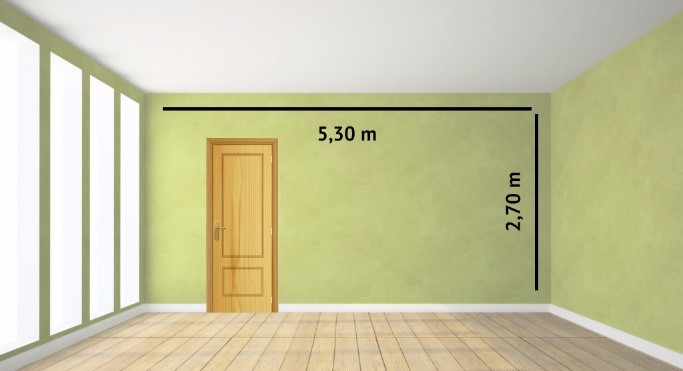
\includegraphics[width=200bp]{superficie11}\hspace{1cm}
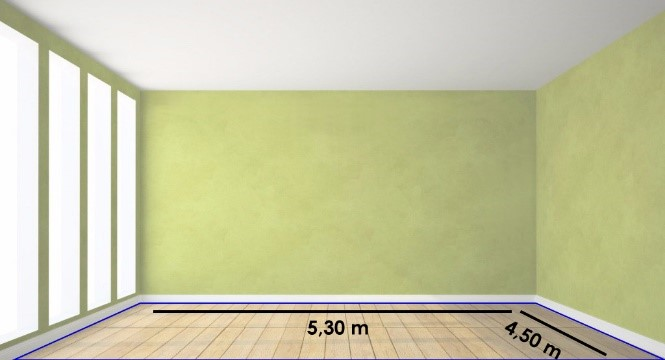
\includegraphics[width=200bp]{superficie12}

\caption{Fonte: \href{https://blog.sincenet.com.br/como-calcular/}{Sincenet}}
\end{figure}

\begin{enumerate}
  \item Calcule a quantidade mínima necessária de cada material, sbendo que Marcelo vai adquirir $10\%$ a mais por segurança e vai dar duas demãos.

  \textbf{Dica}: Consumo de galões = metragem quadrada $\times$ número de demãos $/$ rendimento por lata (informado pelo fabricante).

  \item Calcule o custo total dos materiais.

  \begin{table}[H]
  \centering
  
  \begin{tabu} to \textwidth{|c|c|c|c|}
  \hline
  \thead
  Material & Preço Unitário & Quantidade & Preço Final \\
  \hline
  Piso & R\$ $67{,}00$ a caixa & & \\
  \hline
  Placas de Gesso 3D & R\$ $49{,}90$ por m$^2$ & & \\
  \hline
  Rodapé & R\$ $9{,}38$ por m & & \\
  \hline
  Tinta & R\$ $149{,}90$ a lata ($18\ell$) & & \\
  \hline
  Moldura de Gesso & R\$ $5{,}50$ a peça & & \\
  \hline
  \textbf{Total} & --- & & \\
  \hline
  \end{tabu}
  \end{table}
\end{enumerate}

\end{task}

\begin{task}{empacotamento de latas}
(Atividade adaptada. Fonte: \href{https://m3.ime.unicamp.br/recursos/1009}{IME - Unicamp})

A sociedade moderna já se acostumou com bebidas e alimentos em latas de formato cilíndrico de tamanho apropriado para o uso individual. As indústrias então têm o desafio de transportar grandes quantidades de latas. Para facilitar o transporte é comum pequenos fardos com várias latas e estas são transportadas em caminhões e navios. 

\begin{figure}[H]
\centering

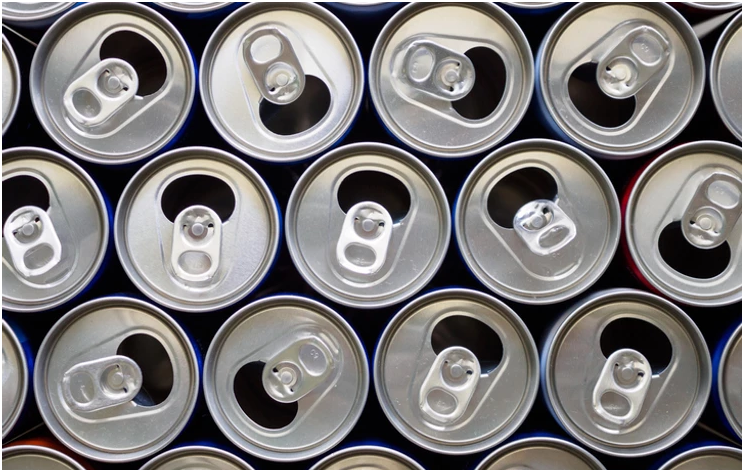
\includegraphics[width=300bp]{superficie13}

\caption{Fonte: \href{https://www.guaranamineiro.com.br/post/latas-de-alumínio-brasil-é-o-maior-reciclador-do-mundo}{Guaraná Mineiro}}
\end{figure}

A matemática tem ferramentas interessantes para otimizar o empacotamento de objetos. Qual será a melhor disposição de forma que o custo para embalar as latas seja o menor possível?

\begin{enumerate}
  \item Escolham três disposições que vocês acham que oferecem os menores custos de embalagem. Registrem no caderno as três disposições escolhidas e numere-as de 1 a 3.
  \item Meça a altura ($h$) e o raio ($r$) da lata. Calcule a área da embalagem utilizada em cada uma das situações.
  	\begin{enumerate}
  	\item Quantidade de latas:
  	\item Altura ($h$):
  	\item Raio ($r$):
  	\item\adjustbox{valign=t}
  	{
  	\begin{tabu} to \textwidth{|c|c|}
  	\hline
  	\thead
  	Disposição & Área (cm$^2$) \\
  	\hline
  	1 & \\
  	\hline
  	2 & \\
  	\hline
  	3 & \\
  	\hline
  	\end{tabu}
  	}
  	\end{enumerate}
  \item Qual das disposiões oferece a embalagem de menor custo?
  \item Com a embalagem de menor custo, calcule o custo de embalagem por lata $A/Q$
\end{enumerate}

\end{task}
\begin{reflection}
Por que a melhor disposição encontrada não é aquela que as empresas usam para embalar as latas?
\end{reflection}

\begin{task}{Retângulos crescentes}
(Atividade adaptada do livro Mentalidades Matemáticas)

\textbf{Parte 1}

Considere um retângulo com $20\text{cm}^2$ de área.

\begin{enumerate}
  \item Qual poderia ser seu comprimento e sua largura? Cite ao menos 5 combinações diferentes.
  \item Agora, amplie cada cada retângulo por um fator escalar $2$.
  \item Liste as dimensões de seus retângulos ampliados e descubra suas áreas. O que você nota?
  \item Desta vez, pense em retângulos ampliados e descubra suas áreas. O que você nota?
  \item Desta vez, pense em retângulos de áreas diferentes e os amplie por um fator escalar $2$.
  \item Você sabe explicar o que está acontecendo?
  \item O que acontece com a área de um retângulo se você o amplia por um fator escalar de 3? E se esse escalar for um número fracionário?
  \item O que acontece com a área de um retêngulo se você o amplia por um fator escalar $k$? Explique e justifique suas conclusões.
\end{enumerate}

\textbf{Parte 2}

Refaça a atividade anterior para outras formas planas, além de reângulos. Explique e justifique suas conclusões.
\end{task}

\arrange{área de figuras planas}

Como já definimos anteriormente, para medir uma porção do plano ocupada por uma figura $F$, devemos compará-la com a unidade de área, e assim o resultado será um número que exprime quantas vezes a figura $F$ contém a unidade de área.

Desse modo, nessa seção vamos organizar essa ideia com um significado mais preciso. Para isso, vamos lembrar das figuras planas mais conhecidas e suas respectivas fórmulas para determinar a sua área.


\subsection{Área do quadrado e do retângulo}

O quadrado é o quadrilátero que tem os 4 lados iguais e os 4 ângulos retos. Se a medida do do lado de um quadrado é $a$, um número real qualquer (inteiro, fracionário ou irracional), sua área é igual a $a^2$, e expressa pela fórmula 
\begin{equation*}
A=a^2.
\end{equation*}

\begin{figure}[H]
\centering

  \begin{tikzpicture}
  \draw [fill=\currentcolor!80] (0,0) rectangle (5,5);
  \draw [\currentcolor!80!black] (0,0) grid (5,5);

  \node [above, overlay] at (2.5,5) {$5$cm};
  \node [right, overlay] at (5,2.5) {$5$cm};
  \end{tikzpicture}

$a=5$cm \hspace{2cm} $A=25$cm$^2$

\caption{Versão interativa: \url{https://www.geogebra.org/m/hsXHDRX7\#material/xpcbYhKT}}
\end{figure}

O retângulo é o quadrilátero que tem os 4 ângulos retos. Se os lados de um retângulo $R$ têm como medidas dois números reais $a$ e $b$, a área de um retângulo é o produto das medidas de seus lados, e expressa pela fórmula 
\begin{equation*}
A=a\times b.
\end{equation*}

\begin{figure}[H]
\centering

  \begin{tikzpicture}
  \draw [fill=\currentcolor!80] (0,0) rectangle (6,4);
  \draw [\currentcolor!80!black] (0,0) grid (6,4);

  \node [above, overlay] at (3,4) {$6$cm};
  \node [right, overlay] at (6,2) {$4$cm};
  \end{tikzpicture}

$a=6$cm,\quad $b=4$cm \hspace{2cm} $A=4\times6=24$cm$^2$

\caption{Versão interativa: \url{https://www.geogebra.org/m/JJDxunvT}}
\end{figure}

\clearpage

\subsection{Área de um paralelogramo}

Conhecida a área de um retângulo, podemos calcular a área de um paralelogramo. O Paralelogramo é um quadrlátero no qual os lados opostos são paralelos. Quando se toma um lado do paralelogramos como base, chama-se altura $a$ um segmento perpendicular que liga a base ao lado oposto (ou aos seu prolongamento).

A área de um paralelogramo é, portanto, o produto da base pela altura, e expressa pela fórmula 
\begin{equation*}
A=b\times h.
\end{equation*}

\begin{figure}[H]
\centering

\begin{tikzpicture}[scale=.9]

\draw [fill=\currentcolor!80] (.5,.5) -- (2.5,4) -- (7.5,4) -- (5.5,.5) -- cycle;
\draw [step=.5, gray!90] (0,0) grid (8,4.5);
\draw (.5,.5) -- (2.5,4) -- (7.5,4) -- (5.5,.5) -- cycle;

\begin{scope}[xshift=8.25cm]

\draw [fill=\currentcolor!80] (.5,.5) -- (2.5,4) -- (7.5,4) -- (5.5,.5) -- cycle;

\begin{scope}
\clip (4,.5) rectangle (7.5,4);
\draw [fill=session2!80] (.5,.5) -- (2.5,4) -- (7.5,4) -- (5.5,.5) -- cycle;
\draw [thick] (4,.5) -- (4,4) node [pos=.5, right] {$h$};

\draw (4,.5) rectangle (4.5,1);
\draw (4,4) rectangle (4.5,3.5);
\end{scope}
\draw [step=.5, gray!80] (0,0) grid (8,4.5);
\draw (.5,.5) -- (2.5,4) -- (7.5,4) -- (5.5,.5) -- cycle;

\end{scope}

\end{tikzpicture}

\end{figure}
\begin{figure}[H]
\centering

\begin{tikzpicture}[scale=.9]

\draw [fill=\currentcolor!80] (.5,.5) rectangle (5.5,4);
\draw [thick] (2,.5) -- (4,4); 
\draw (.5,.5) rectangle (1,1);
\draw (.5,4) rectangle (1,3.5);

\node [right] at (.5,2) {$h$};

\begin{scope}
\clip (2,.5) -- (4,4) -- (.5,4) -- (.5,.5) -- cycle;
\draw [fill=session2!80] (.5,.5) rectangle (7.5,4);
\end{scope}
\draw [step=.5, gray!90] (-1,0) grid (7,4.5);
\draw (.5,.5) rectangle (5.5,4);

\end{tikzpicture}

\caption{Versão interativa: \url{https://www.geogebra.org/m/R42DVZ8K\#material/D8rjsGzF}}
\end{figure}

\subsection{Área de um triângulo}

Da área de um paralelogramo, passamos imediatamente par a área de um triângulo, pois todo triângulo é a metade de um paralelogramo.

Assim, a área de um triângulo é, portanto, a metade do produto da base pela altura, e expressa pela fórmula 
\begin{equation*}
A=\frac{b\times h}{2}.
\end{equation*}

\begin{figure}[H]
\centering


\begin{tikzpicture}[scale=.9]

\draw [fill=\currentcolor!80] (.5,.5) -- (2.5,4) -- (5.5,.5) -- cycle;

\end{tikzpicture}\quad
\begin{tikzpicture}[scale=.9]

\draw [fill=\currentcolor!80] (.5,.5) -- (2.5,4) -- (7.5,4) -- (5.5,.5) -- cycle;
\draw (2.5,4) -- (5.5,.5);

\end{tikzpicture}


\caption{Versão interativa: \url{https://www.geogebra.org/m/R42DVZ8K\#material/uKQKXvu3}}
\end{figure}

\textbf{Obs.}: Observe que em um triângulo temos 3 opções para base $b$ e, portanto, três opções para a altura $h$. Em qualquer uma das opções sempre teremos o dobro da área do triângulo. Dessa forma, a área de um triângulo não se altera quando sua base permanece fixa e o vértice oposto percorre uma reta paralela à base.

\begin{figure}[H]
\centering

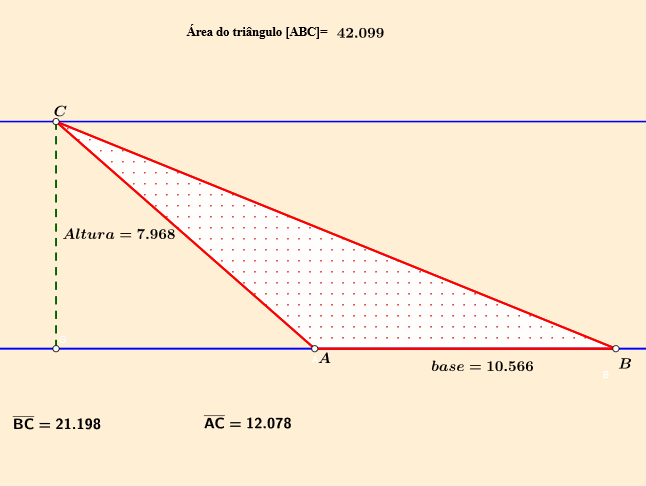
\includegraphics[height=135bp]{superficie21}\hspace{1em}
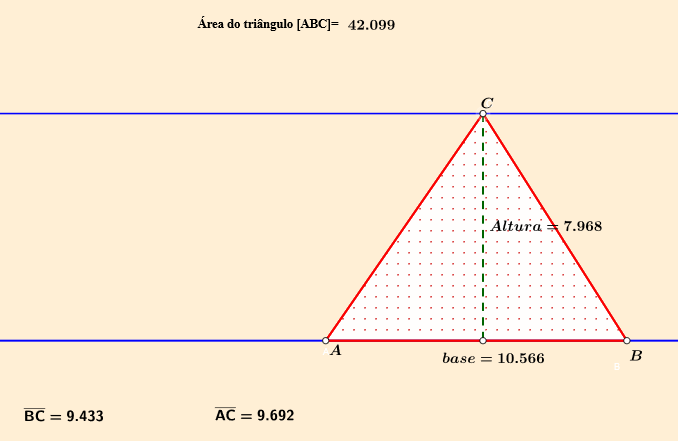
\includegraphics[height=135bp]{superficie22}

\caption{Versão interativa: \url{https://www.geogebra.org/m/uq5VxUcW}}
\end{figure}

\subsection{ Área de um trapézio}

Chamamos de base média de um trapézio ao segmento de reta que une os pontos médios dos lados não paralelos. Sua medida é a média aritmética das medidas das bases.

A área do trapézio é o produto da base média pela altura, expressa pela fórmula 
\begin{equation*}
A=\frac{(b+b)\times h}{2}.
\end{equation*}

\begin{figure}[H]
\centering

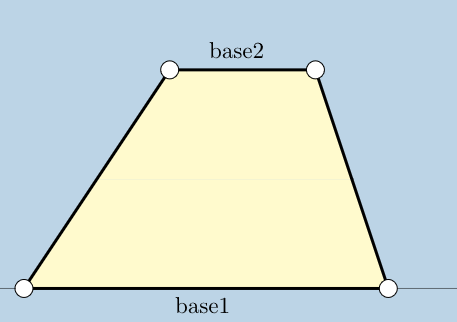
\includegraphics[height=85bp]{superficie23}\hspace{.5em}
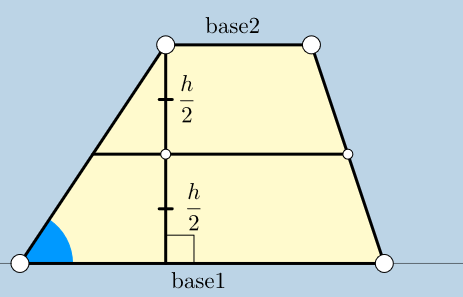
\includegraphics[height=85bp]{superficie24}\hspace{.5em}
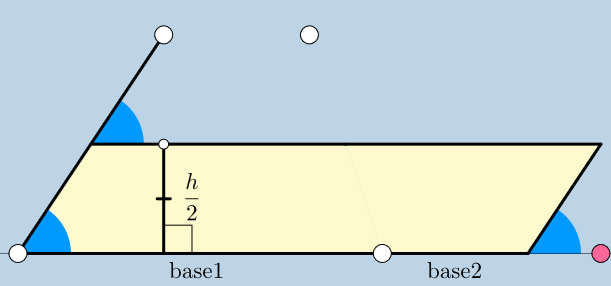
\includegraphics[height=85bp]{superficie25}

\caption{Versão interativa: \url{https://www.geogebra.org/m/R42DVZ8K\#material/rktj8gqv}}
\end{figure}

\subsection{ Área de um losango}

Um losango é um quadrilátero que tem os lados com medidas iguais. A área do losango é a metade do produto das medidas de suas diagonais, expressa pela fórmula  
\begin{equation*}
A=\frac{D\times d}{2}.
\end{equation*}

\begin{figure}[H]
\centering

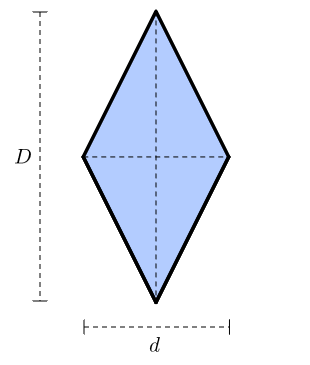
\includegraphics[height=135bp]{superficie26}\hspace{.5em}
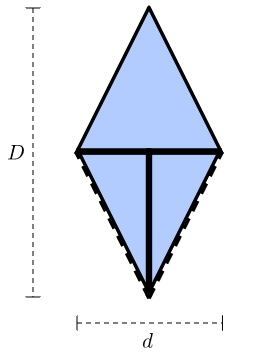
\includegraphics[height=135bp]{superficie27}\hspace{.5em}
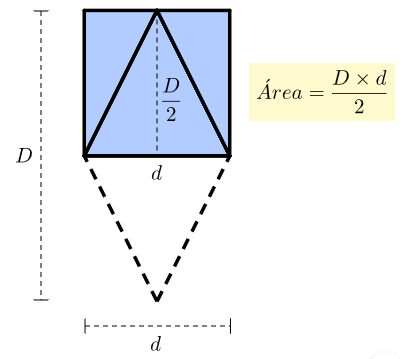
\includegraphics[height=135bp]{superficie28}

\caption{Versão interativa: \url{https://www.geogebra.org/m/fUEGv6D6}}
\end{figure}

Para um polígono qualquer, para calcular a sua área, podemos subdividi-lo em figuras tais como triângulos, quadriláteros ou outra qualquer cuja área sabemos calcular. Desta forma, a área do polígono procurado será a soma das áreas das figuras em que o decompusemos.

\subsection{ Área de um hexágono regular}

Para o cálculo da área de qualquer polígono regular basta calcularmos a área de um dos triângulos isósceles a partir do centro do polígono e multiplicá-la pelo número de lados do polígono.

\begin{multicols}{2}
\centering
Área do triângulo equilátero: 
\begin{equation*}
A=\frac{l^2\sqrt{3}}{4}.
\end{equation*}

Área do triângulo equilátero: 
\begin{equation*}
A=6\times\frac{l^2\sqrt{3}}{4}
\end{equation*}
\end{multicols}

\begin{figure}[H]
\centering

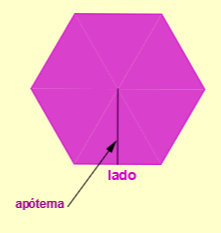
\includegraphics[height=85bp]{superficie29}\hspace{1em}
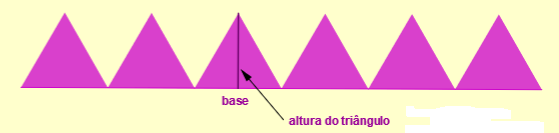
\includegraphics[height=85bp]{superficie30}

\caption{Versão interativa: \url{https://www.geogebra.org/m/RgAY5xdQ}}
\end{figure}

\textbf{Área do círculo}

A área de um círculo de raio $r$ é uma função desse raio. Então a área de um círculo de raio $r$ é expressa pela fórmula
\begin{equation*}
A=\pi r^2.
\end{equation*}

\begin{figure}[H]
\centering

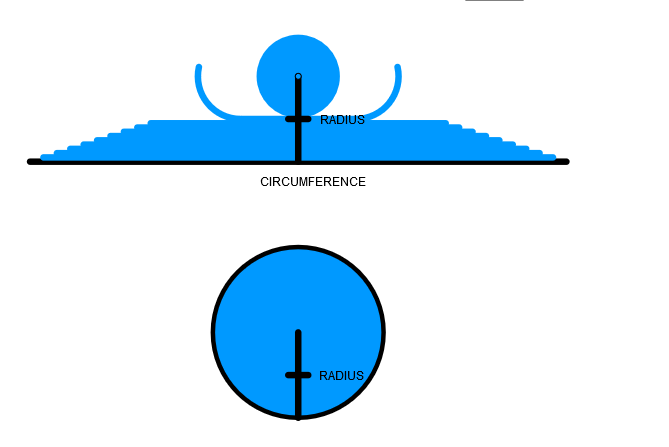
\includegraphics[height=125bp]{superficie31}\hspace{1em}
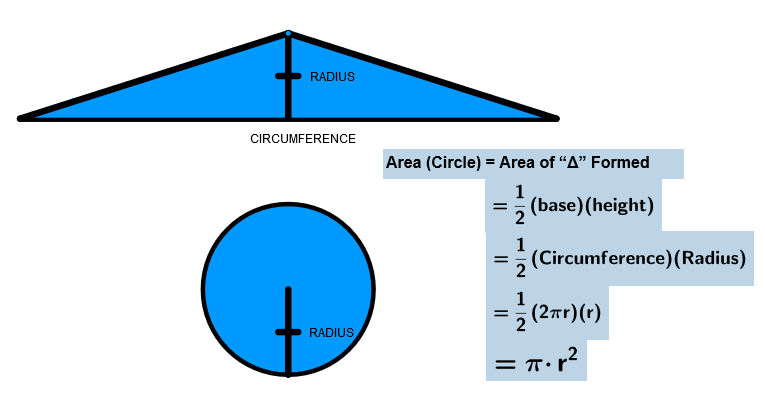
\includegraphics[height=125bp]{superficie32}

\caption{Versão interativa: \url{https://www.geogebra.org/m/R42DVZ8K\#material/Ga3e6tfV}}
\end{figure}

\clearpage

\practice{Área de figuras planas}

\begin{task}{reforma da piscina}

Uma piscina tem $10$m de comprimento, $6$m de largura e $1{,}6$m de profundidade. Determine quantos ladrilhos quadrados de $20$cm de lado são necessários para ladrilhar essa piscina.

\begin{figure}[H]
\centering

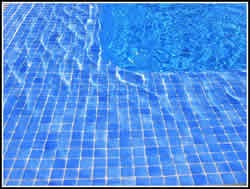
\includegraphics[width=175bp]{superficie33}

\end{figure}
\end{task}

\begin{task}{Quadra de basquete 3$\bm{\times}$3}

Uma das novidade na programação das Olimpíadas de Tóquio será o bastquete $3\times3$. Essa modalidade surgiu com fote influência da prática do esporte nas ruas, que tem como principais características, a disputa acirrada no placar e a participação dos jovens com jogadas de efeito. Marcelo quer mobilizar seus amigos para construir uma quadra de basquete $3\times3$, na sua comunidade. Para isso resolveu fazer um esboço da quadra e calcular a área correspondente a cada cor.

\begin{figure}[H]
\centering

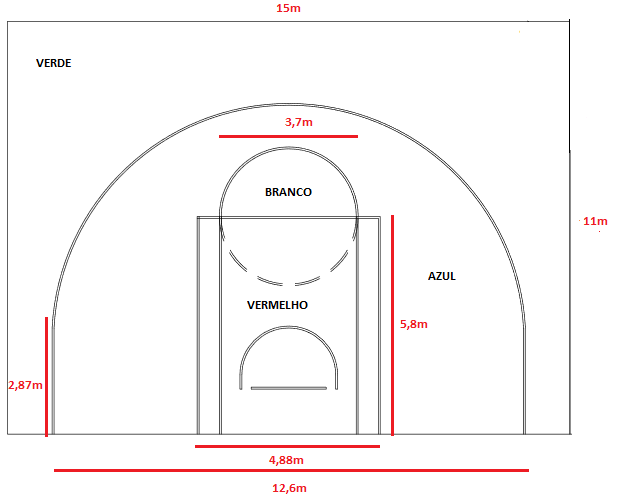
\includegraphics[width=325bp]{superficie35}

\end{figure}

Marcelo e seus amigos conseguiram arrecadar R\$$350{,}00$. Ele ainda descobriu que uma lada de $3{,}6$ litros custa $\$68{,}60$ e tem um rendimento de aproximadamente $70$m$^2$. A tinta é à base de resina acrílica para pisos cimentados, mesmo que já tenham sido pintados anteriormente. Tem grande poder de cobertura e alta durabilidade. Por isso, é muito resistente ao tráfego de pessoas, carros e intempéries, quando aplicada sobre superfícies corretamente preparadas e conservadas. Deve ser passado duas a três demãos %\url{https://loja.politintas.com.br/tinta-novacor-piso-mais-resistentesherwin-williams-3-6l/p#}
. Verifique a quantidade de tinta necessária, sabendo que vão passar duas demãos, e se é possível comprar com o valor que já foi arrecadado. Use $\pi=3{,}14$.
\end{task}

\begin{task}{a praça}
(Atividade adaptada da OBMEP - 2005)

Um prefeito quer construir uma praça quadrada de $10$m de lado, que terá canteiros triangulares iguais de pedra e um canteiro quadrado de grama, como na figura. O prefeito ainda não decidiu qual será a área do canteiro de grama, por isso o comprimento deste segmento $AB$ está indicado por $x$ na figura.

\begin{figure}[H]
\centering

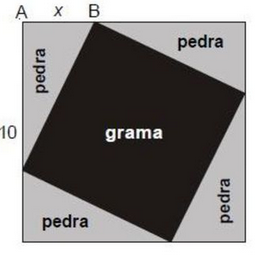
\includegraphics[width=.3\textwidth]{superficie36}
\end{figure}
\clearpage
\begin{enumerate}
  \item Calcule a área do canteiro de grama para $x=2$.
  \item Escreva a expressão da área do canteiro de grama em função de $x$.
  \item Sabe-se que o canteiro de grama custa R\$$4{,}00$ por metro quadrado, e os canteiros de pedra custam R\$$3{,}00$ por metro quadrado. Qual a menor quantia que o prefeito deve ter para construir os cinco canteiros?
\end{enumerate}
\end{task}

\begin{task}{Arcos de circunferência}
(UFSCar-SP) Considere a região $R$ pintada de preto exibida a seguir, construída no interior de um quadrado de lado medindo $4$cm.

\begin{figure}[H]
\centering

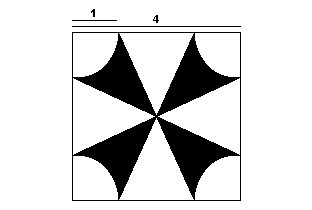
\includegraphics[width=150bp]{superficie38}
\end{figure}

Sabendo-se que os arcos de circunferência que aparecem nos cantos do quadrado têm seus centros nos vértices do quadrado e que cada raio mede $1$cm, determine a área da região $R$.
\end{task}

\explore{composição; decomposição; planificação}

\begin{task}{comparando embalagens}

Uma marca de leite condensado comercializa seus produtos em duas embalagens diferentes, mas ambas com $395$g. A embalagem cilíndrica tem $6{,}5$cm de diâmetro na base e $\times$ $9{,}5$cm de altura, e a outra embalagem tem a forma de um paralelepípedo retângulo de medidas $6{,}2\text{cm}\times4{,}0\text{cm}\times12{,}0\text{cm}$.

\begin{figure}[H]
\centering

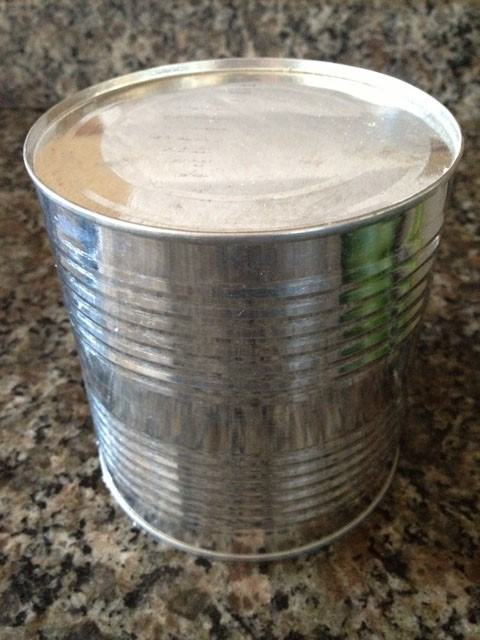
\includegraphics[height=200bp]{superficie39}\hspace{1cm}
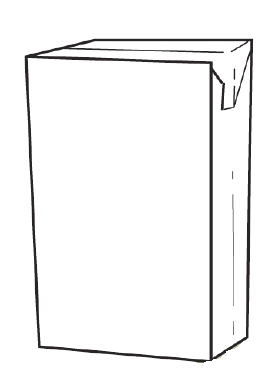
\includegraphics[height=200bp]{superficie40}

\end{figure}

Qual das embalagens apresenta a menor quantidade de material?

\end{task}
\begin{task}{almofada para leitura}
Helena gosta muito de ler na sua cama e está procurando uma almofada que lhe dê  mais conforto. Aos pesquisar na internet encontrou a seguinte descrição:

\begin{wrapfigure}[10]{l}{.35\textwidth}
\vspace{-1em}
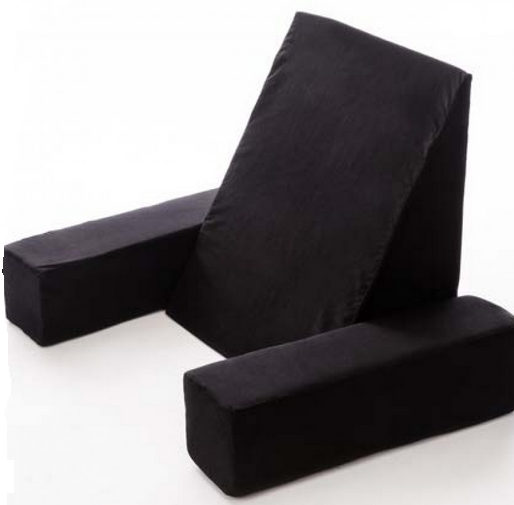
\includegraphics[width=.35\textwidth]{superficie41}
\end{wrapfigure}
\textit{"A almofada triangular é indicada para acomodar melhor o usuário na cama ou sofá, proporcionando maior conforto e diminuindo as dores nas costas. Pode ser utilizada para assistir tv e para leitura. Em pós cirúrgico para manter o tronco elevado em relação a parte inferior ou mesmo os pés mais elevado para auxiliar na circulação sanguínea e também para pessoas que necessitam passar por longos períodos em uma cama sem movimento fowler, elevação de cabeça e pés"}
\flushright
(\href{https://www.mobraz.com.br/produto/almofada-triangular-para-leitura-perfetto}{Loja Mobraz})
\clearpage

\justify
Como ela conhece uma costureira muito criativa, enviou a foto e as seguintes medidas:
\begin{itemize}
  \item Dimensões da almofada de encosto: $43\text{cm}\times50\text{cm}\times30\text{cm}$;
  \item Dimensões do apoio de braço: $13\text{cm}\times10\text{cm}\times50\text{cm}$
\end{itemize}
\noindent Calcule a quantidade mínima de tecido que Helena deve levar para a costureira.
\end{task}

\begin{task}{a barraca de camping}
O Movimento Escoteiro foi fundado em 1907, na Inglaterra, por Robert Baden-Powell, condecorado militar britânico que iniciou como uma proposta de atividades ao ar livre para grupos de jovens na Inglaterra do início do século vinte, hoje segue em constante atualização no mundo em que vivemos, com foco principal no protagonismo e no envolvimento juvenil. Através de um programa educativo baseado na Lei e na Promessa Escoteira, o escotismo foi, e ainda é, um dos maiores movimentos de educação não formal para jovens do mundo. 

O escotismo pode ser considerado como um grande jogo ao ar livre, onde os jovens dividem-se em pequenos grupos, as patrulhas ou matilhas, e realizam diversas atividades que lhes dão a oportunidade de desenvolver habilidades e conhecimentos. São acampamentos, jornadas, trilhas, aventuras e desafios em grupo que a cada dia os tornam mais empoderados e cientes das suas responsabilidades, tornando-os cidadãos ativos dentro e fora do escotismo.

\begin{figure}[H]
\centering

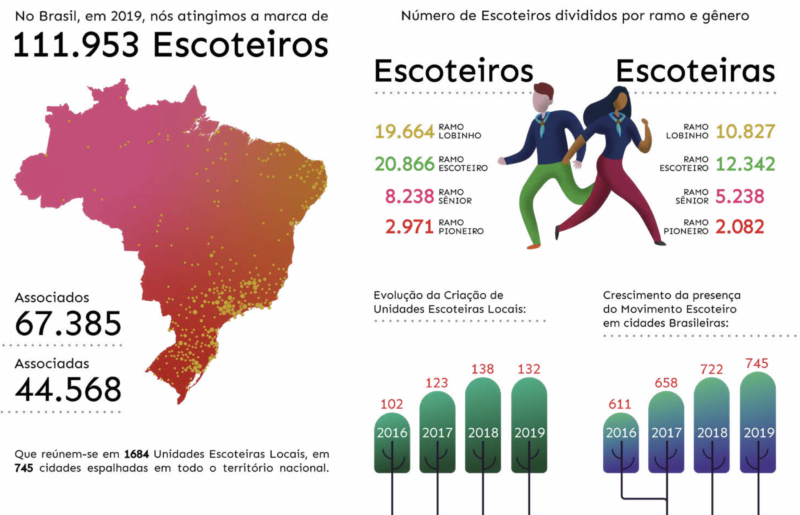
\includegraphics[width=325bp]{superficie42}

\caption{Fonte: \href{https://www.escoteiros.org.br/wp-content/uploads/2020/07/1.1.1-Foto-Gráfico-1-800x515.png}{Escoteiros do Brasil}}
\end{figure}

João e Luiza são da tropa Sênior. O Ramo Sênior é formado por jovens com idades entre 15 e 17 anos, que incentiva a superar os próprios desafios! Com a tropa sênior vivemos verdadeiras aventuras: fazemos rapel, navegamos, acampamos por vários dias, fazemos trilhas e escaladas, aprendemos jogos e atividades mais desafiadoras e somos incentivados a superar obstáculos.

Como parte do seu desafio, você ainda vai precisar de 10 noites acampado com sua patrulha ou tropa do Ramo Sênior, conquistar o cordão dourado, uma das Insígnias de Interesse Especial e uma das Insígnias da Modalidade do seu atual Ramo. Ao chegar no acampamento, a tropa foi surpreendida pelo desafio "\textit{Apresente a área total de sua barraca em m$^2$. O primeiro que acertar o resultado ganha o prêmio de 100 pontos}". Sabendo que a barraca de João e Luiza está apresentada na figura abaixo, determine a área total da barraca.
\begin{figure}[H]
\centering

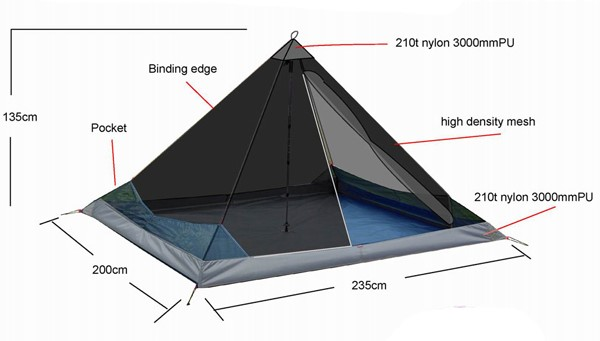
\includegraphics[width=350bp]{superficie43}
\end{figure}
\end{task}

\begin{task}{Quanto você tem de pele?}
(Atividade adaptada de \href{https://m3.ime.unicamp.br/recursos/1032}{IME-Unicamp})

\begin{wrapfigure}[10]{r}{.4\textwidth}
\vspace{-1.2em}
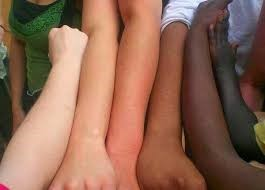
\includegraphics[width=.4\textwidth]{superficie44}

\caption{Fonte: \href{https://escolaeducacao.com.br/pele-humana/}{Escola Educação}}
\end{wrapfigure}

A pele é o maior órgão do corpo humano. Ela acumula várias funções como proteção, regulação da temperatura e armazenamento de energia. Além disso, a pele é responsável por grande parte das informações que recebemos do ambiente ao nosso redor, isto é, as sensações de calor, pressão e tato, sem as quais nossa vida seria muito mais complicada. 

Já imaginou as consequências de não sentir o calor do fogo? Mas qual será o tamanho deste órgão que tem tantas funções importantes? Este será o desafio do experimento: calcular a área da superfície da pele humana.


\begin{enumerate}
  \item Como podemos medir a área da pele? Discuta com seu grupo e registre.
  \item Aproxime cada parte do corpo a um sólido de área de superfície conhecida. Discuta os resultados com a turma.

  \begin{table}[H]
  \centering
  
  \begin{tabu} to \textwidth{|c|c|}
  \hline
  \thead
  Partes do corpo & Forma geométrica semelhante \\
  \hline
  & \\
  \hline
  & \\
  \hline
  & \\
  \hline
  & \\
  \hline
  & \\
  \hline
  & \\
  \hline
  & \\
  \hline
  \end{tabu}
  \end{table}
  \item Escolha um membro do grupo para ser o modelo
  \begin{itemize}
    \item Decida qual sólido geométrico representará cada parte do corpo do modelo.
    \item Quais medidas são necessárias para obter a área da superfície de cada sólido?
  \end{itemize}
  \item Agora, meça o modelo do grupo e calcule a área da superfície de cada sólido escolhido por vocês.
  \begin{table}[H]
  \centering
  
  \begin{tabu} to \textwidth{|c|c|c|}
  \hline
  \thead
  Sólido Geométrico & Fórmula para a área de superfície & Valor obtido da área \\ 
  \hline
  & & \\
  \hline
  & & \\
  \hline
  & & \\
  \hline
  & & \\
  \hline
  & & \\
  \hline 
  & & \\
  \hline
  & & \\
  \hline
  \tmcol{2}{|c|}{Área total da superfície da pele} & \\
  \hline
  \end{tabu}
  \end{table}
\end{enumerate}

\begin{reflection}
O método de medida da área da superfície da pele, comumente usada pelos médicos, foi desenvolvido por Frederick Mosteller (1916-2006), usando a fórmula
\begin{equation*}
A=\frac{\sqrt{h\cdot m}}{60},
\end{equation*}
onde $h$ é a altura em centímetros e $m$ é a massa em quilogramas.

Calcule a área da pele de todos os componentes do grupo usando a fórmula acima. Analise os resultados obtidos com a fórmula desenvolvida por Mosteller e o valor calculado para o aluno modelo.
\end{reflection}

\end{task}

\arrange{composição; decomposição; planificação}
Para calcular a área de um polígono qualquer, basta subdividi-lo em figuras tais como triângulos, quadriláteros ou outra qualquer cuja área sabemos calcular. Desta forma, a área do polígono procurado será a soma das áreas das figuras em que o decompusemos.

Assim, o cálculo de áreas de polígonos segue as seguintes regras:
\begin{enumerate}[label=\titem{\arabic*)}]
  \item Podemos associar cada polígono $P$ um número real positivo chamado área de $P$.
  \item A área de um quadrado de lado unitário é igual a $1$.
  \item Polígonos congruentes têm áreas iguais.
  \item Se um polígono $P$ está decomposto em outros polígonos, de forma que dois quaisquer possuam em comum, no máximo pontos de seus lados, então a área de $P$ é a soma das áreas desses polígonos.
\end{enumerate}

Note que as fórmulas da seção anterior foram deduzidas a partir das propriedades acima. Se sabemos que podemos encontrar a área de uma figura plana, você acha que é possível encontrar a área de uma superficie? De fato, o que é a área de uma superfície?

Área de superfície é a área da superfície da forma tridimensional. Quase todos os objetos tridimensionais com os quais você lida são compostos de faces bidimensionais(figuras planas) que são apenas quadrados, triângulos etc., e os que são curvados como esferas terão suas próprias fórmulas especiais para a área de superfície.

\subsection{Área da superfície de prismas retos}

Prismas retos são prismas obtidos tomando, para as arestas laterais, retas perpendiculares ao plano da base. Como consequência, as faces lateriais são retângulos.
\begin{figure}[H]
\centering

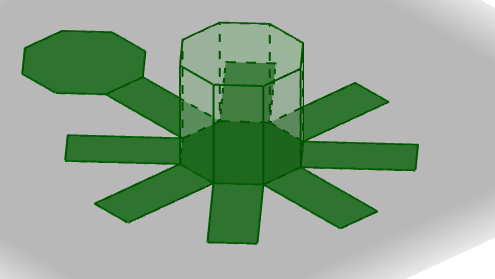
\includegraphics[width=250bp]{superficie45}

\caption{Versão interativa: \url{https://www.geogebra.org/m/uz5ddyzy}}
\end{figure}

Desse modo, convencionaremos:
\begin{itemize}
  \item $A_b$: área da base -- depende do polígono da base.
  \item $A_l$: área lateral -- é a soma das áreas de retângulos cujas medidas são respectivamente as de um lado do polígono da base  ($l$) e a altura do prisma ($h$), tantas quantas forem os lados do polígono da base. Expressamos por 
  \begin{equation*}
  A_l=n\times l\times h.
  \end{equation*}
  \item $A_t$: área total da superfície -- é a soma das áreas das bases e da área lateral. Expressamos por 
  \begin{equation*}
  A_t=2A_b+A_l
  \end{equation*}
\end{itemize}

Há diversos casos particulares importantes;

\begin{itemize}
  \item Quando a base é um polígono regular, obtemos um prisma regular
  \begin{figure}[H]
  \centering

  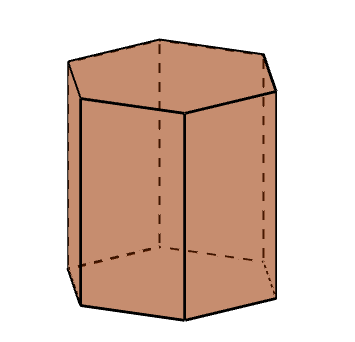
\includegraphics[width=125bp]{superficie46}\hspace{.5em}
  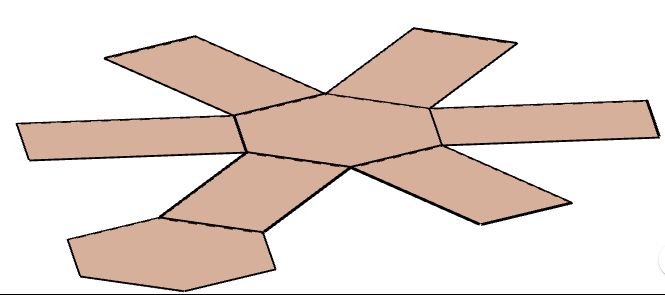
\includegraphics[width=200bp]{superficie47}

  \caption{Versão interativa: \url{https://www.geogebra.org/m/Fpjf6QRq}}
  \end{figure}

  \item Quando a base é um retângulo, obtemos um paralelepípedo retângulo, onde cada face é um retângulo, assim qualquer face serve como base.
  \begin{figure}[H]
  \centering

  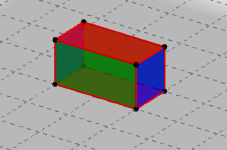
\includegraphics[height=80bp]{superficie48}\hspace{.5em}
  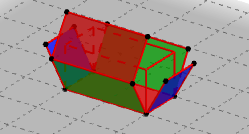
\includegraphics[height=80bp]{superficie49}\hspace{.5em}
  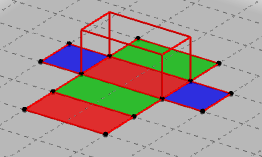
\includegraphics[height=80bp]{superficie50}

  \caption{Versão interativa: \url{https://www.geogebra.org/m/k8kKsFUz}}
   \end{figure}

   \item Quando a base é um quadrado e as arestas possuem a mesma medida do lado da base, obtemos um hexaedro regular (ou cubo)

   \begin{figure}[H]
   \centering

   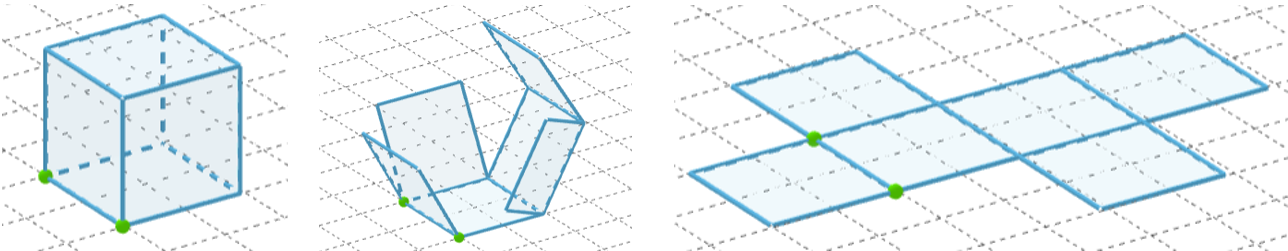
\includegraphics[width=350bp]{superficie51}


   \caption{Versão interativa: \url{https://www.geogebra.org/m/dyz3zBwn}}
   \end{figure}
\end{itemize}

\subsection{ Área da superfície de cilindros retos}

O cilindro é chamado reto no caso em que suas geratrizes são perpendiculares aos planos das bases. O cilindro equilátero é o cilindro circular reto em que a altura é igual ao diâmetro da base.

\begin{figure}[H]
\centering

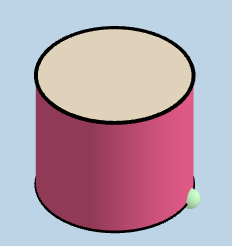
\includegraphics[height=100bp]{superficie52}\hspace{.5em}
\includegraphics[height=100bp]{superficie53}\hspace{.5em}
\includegraphics[height=100bp]{superficie54}

\caption{Versão interativa: \url{https://www.geogebra.org/m/XzfFNDYV}}
\end{figure}

Desse modo, convencionaremos:
\begin{itemize}
  \item $A_b$: área da base -- área do círculo. Expressamos por
  \begin{equation*}
  A_b=\pi r^2,
  \end{equation*}
  onde $r$ é o raio do cilindro

  \item $A_l$: área lateral -- a superfície lateral de um cilindro reto de raio $r$ e altura $h$, pode ser desenrolada e transformada em um retângulo de base $2\pi r$ e altura $h$. A área lateral do cilindro é igual à área desse retângulo, e expressamos por  
  \begin{equation*}
  A_l=2\pi rh.
  \end{equation*}
  \item $A_t$: área total da superfície -- é a soma das áreas das bases e da área lateral. Expressamos por 
  \begin{equation*}
  A_t=2A_b+A_l=2\pi r^2+2\pi rh=2\pi r(r+h)
  \end{equation*}
\end{itemize}

O cilindro circular reto é também chamado de cilindro de revolução, por ser gerado pela rotação completa de um retângulo por um de seus lados. Assim, a rotação do retângulo pelo lado gera o cilindro mostrado.

\begin{figure}[H]
\centering

\includegraphics[height=150bp]{superficie55}\hspace{.5em}
\includegraphics[height=150bp]{superficie56}\hspace{.5em}
\includegraphics[height=150bp]{superficie57}

\caption{Versão interativa: \url{https://www.geogebra.org/m/nh2xNMe7}}
\end{figure}

\subsection{ Área da superfície de pirâmides retas}

Uma pirâmide reta é aquela cuja projeção ortogonal do vértice sobre o plano da base é o centro da base.

\begin{figure}[H]
\centering

\includegraphics[height=150bp]{superficie58}\hspace{.5em}
\includegraphics[height=150bp]{superficie59}

\caption{Versão interativa: \url{https://www.geogebra.org/m/cdxwhx4t}}
\end{figure}

Desse modo, convencionaremos:
\begin{itemize}
  \item $A_b$: área da base -- depende da figura que temos como polígono da base.
  \item $A_l$: área lateral -- a superfície lateral de uma pirâmide é formada por $n$ triângulos cuja base tem a mesma medida do lado do polígono da base, e a altura é o apótema (A) da face lateral da pirâmide. A área lateral da pirâmide é igual à $n$ vezes a área desse triângulo, e expressamos por
  \begin{equation*}
  A_l=\frac{nAl}{2}.
  \end{equation*}
  \item $A_t$: área total da superfície -- é a soma das áreas das bases e da área lateral. Expressamos por 
  \begin{equation*}
  A_t=A_b+A_l
  \end{equation*}
\end{itemize}

Pirâmide regular é uma pirâmide cuja base é um posígosno regular e a projeção ortogonal do vértice sobre o plano da base é o centro da pirâmide. Uma pirâmide regular possui arestas laterais congruentes e as faces laterais são triângulos isósceles.

\begin{figure}[H]
\centering

\includegraphics[height=150bp]{superficie60}\hspace{.5em}
\includegraphics[height=150bp]{superficie61}
\end{figure}

Dessa forma, valem as seguintes relações para as pirâmides regulares retas, quando a apótema do triângulo isósceles que seja uma face lateral é também chamado de geratriz da pirâmide:
\begin{itemize}
  \item $(a_l)^2=A^2+\bigg(\dfrac{l}{2}\bigg)^2$, onde $a_l$ representa a aresta lateral, $A$ é a geratriz ou apótema e $l$, é o lado da base.
  \item $A^2=h^2+a^2$, onde $a$ representa o apótema da base, $A$ é a geratriz ou apótema, e $h$ é a altura da pirâmide.
\end{itemize}

\begin{figure}[H]
\centering

\includegraphics[height=150bp]{superficie62}
\end{figure}

\subsection{ Área da superfície de cones retos}

Em um cone, a base não precisa ser um polígono, mas qualquer região plana delimitada por uma curva fechada. Os cones mais importantes são os cones circulares, em que a base é um círculo. Um cone é equilátero quando a medida da geratriz é igual à medida do diâmetro da base.

\begin{figure}[H]
\centering

% \resizebox{\textwidth}{!}
{\includegraphics[height=100bp]{superficie63}\hspace{.5em}
\includegraphics[height=100bp]{superficie64}\hspace{.5em}
\includegraphics[height=100bp]{superficie65}}

\caption{Versão interativa: \url{https://www.geogebra.org/m/yzGzrUxs}}
\end{figure}

Desse modo, convencionados

\begin{itemize}
  \item $A_b$: área da base -- área do círculo de raio $r$. Expressamos por
  \begin{equation*}
  A_b=\pi r^2
  \end{equation*}  
  \item $A_l$: área lateral -- a superfície lateral de um cone de raio $r$ e geratriz $g$, pode ser desenrolada e transformada em um setor de raio $g$, cujo arco tem comprimento $2\pi r$. A área deste setor é igual à área lateral do cone, e para calculá-la usaremos proporcionalidade. Diremos que
  \begin{equation*}
  \frac{\text{área do setor}}{\text{área do círculo}}=\frac{\text{comprimento do arco}}{\text{comprimento da circunferência}},
  \end{equation*}
  ou ainda,
  \begin{equation*}
  \frac{A_l}{\pi g^2}=\frac{2\pi r}{2\pi g}.
  \end{equation*}
  Expressamos por $A_l=\pi rg$.
  \item $A_t$: área total da superfície -- é a soma da área da base e da área lateral. Expressamos por
  \begin{equation*}
  A_t=A_b+A_l=\pi r^2+\pi rg=\pi r(r+g).  
  \end{equation*}
\end{itemize}

Um cone circular reto também é chamado de cone de revolução, por ser gerado pela rotação de um triângulo retângulo em torno do eixo dado por um dos catetos.

\begin{figure}[H]
\centering

\includegraphics[height=125bp]{superficie66}\hspace{.5em}
\includegraphics[height=125bp]{superficie67}\hspace{.5em}
\includegraphics[height=125bp]{superficie68}

\caption{Versão interativa: \url{https://www.geogebra.org/m/deyt2w4u}}
\end{figure}

Para o cone reto, todos os segmentos que formam sua superfície lateral têm a mesma medida. Esse segmento comum é a geratriz do cone, denotada por $g$ e sua medida, e sua medida satisfaz a relação 
\begin{equation*}
g^=h^2+r^2
\end{equation*}

Vamos considerar o tronco de cone reto como sendo a parte do cone compreendida entre o plano que contém a base do cone e outro plano paralelo a esse, que secciona o cone. A base do tronco é o círculo de raio $R$ e o topo é um círculo de raio $r$. Sua altura é o segmento perpendicular à base entre os dois planos. A geratriz $g$ do tronco é o segmento da geratriz $G$ do cone, compreendido entre o topo e a base.
\begin{figure}[H]
\centering

\includegraphics[width=250bp]{superficie69}

\caption{Versão interativa: \url{https://m3.ime.unicamp.br/recursos/1032}}
\end{figure}

Então, a área $A_t$ da superfície de um tronco de cone pode ser calculada como a diferença entre a área da superfície do cone inicial e a área da superfície do cone que restou após ser retirado o tronco. Veja na figura abaixo:

\begin{figure}[H]
\centering

\includegraphics[width=400bp]{superficie71}

\caption{Fonte: \href{https://m3.ime.unicamp.br/recursos/1032}{IME-Unicamp}}
\end{figure}
% \begin{figure}[H]
% \centering

% \begin{tikzpicture}
% \coordinate (A) at (0,0);
% \coordinate (V) at (0,4);
% \coordinate (B) at (2,0);
% \coordinate (G) at (1.5,3);

% \draw (A) -- (V) -- (B) -- cycle;
% \draw (G) -- +($(B)!(G)!(V)$);

% \node [fill=white] at (1.5,3) {$G$};
% \end{tikzpicture}
% \end{figure}

Assim,
\begin{equation*}
A_t=\pi(R+r)g
\end{equation*}

\subsection{ Área da superfície da esfera}

A área da superfície da esfera de raio $R$ é igual a 

\begin{equation*}
4\pi R^2.
\end{equation*}

Uma ideia para se chegar a essa fórmula é considerar a superfície da esfera como o resultado da rotação de uma semicircuferência em dorno de seu eixo.

Imaginemos a esfera dividida em infinitas \textit{cunhas} e cada uma dessas cunhas dividida em infinitas pirâmides de altura $h$ igual ao raio $r$ da esfera.

Sejam ainda $A_1,A_2,A_3,...,A_n$ as áreas das bases de cada uma dessas pirâmides.

Lembrando que

\begin{align*}
V_{\text{esf}}&=\frac{4}{3}\pi r^3\\
V_{\text{pir}}=&\frac{1}{3}A_bh.
\end{align*}

Como o volume total das pirâmide é aproximadamente o volume da esfera,

\begin{align*}
&\frac{1}{3}A_1 r+\frac{1}{3}A_2 r+\frac{1}{3}A_3r+\cdots\frac{1}{3}A_n r \approx\frac{4}{3}\pi r^3\\
&\frac{1}{3}r(A_1,+A_2+A_3+\cdots+A_n)\approx\frac{4}{3}\pi r^3.
\end{align*}

Quando $n$ tende a infinito,

\begin{align*}
\frac{1}{3}rS_3\approx\frac{4}{3}\pi r^3\\
\therefore S_3\approx4\pi r^2
\end{align*}
\begin{figure}[H]
\centering

\includegraphics[width=350bp]{superficie73}

\caption{Versão interativa: \url{https://www.geogebra.org/m/nrcwwbg3}}
\end{figure}

\practice{composição; decomposição; planificação}


\begin{task}{Planetário}

(UFSM - 2011) Oscar Niemayer é um arquiteto brasileiro, considerado um dos nomes mais influentes na arquitetura moderna internacional. Ele contribuiu, através de uma doação de um croqui, para a construição do planetário da UFSM, um marco arquitetônico importante da cidade de Santa Maria.

\begin{figure}[H]
\centering

\includegraphics[width=275bp]{superficie76}

\end{figure}

Suponha que a cobertura da construção seja uma semiesfera de $28$m de diâmetro, vazada por 12 parte iguais, as quais são aproximadas por semicírculos de raio $3$m. Sabendo que uma lata de tinta é suficiente para pintar $39\text{m}^2$ de área, qual a quantidade mínima de latas de tinta necessária para pintar toda a cobertura do planetário? (use $\pi=3$).

\end{task}

\begin{task}{telhado}
\begin{wrapfigure}{r}{.5\textwidth}
\centering
\includegraphics[width=.5\textwidth]{superficie77}

\end{wrapfigure}
(PUC RS/2012) A quantidade de materiais para executar uma obra é essecial para prever o custo da construção. Quer-se construir um telhado cujas dimensões e formato são indicados na figura abaixo.

A quantidade de telhas de tamanho $15$cm por $20$cm necessárias para fazer esse telhado é:


\end{task}

\clearpage

\begin{task}{comprimidos de remédios}

(Faap) A razão na qual um comprimido de vitamina C começa a dissolver-se depende da área da superfície do comprimido. Uma marca de comprimido tem forma cilíndrica, comprimento $2$ centímetros, com hemisférios de diâmetro $0{,}5$ centímetro cada extremidade, conforme a figura a seguir. Uma segunda marca de comprimido avai ser fabricada em forma cilíndrica, com $0{,}5$ centímetro de altura.

\begin{wrapfigure}{r}{.4\textwidth}
\centering

\includegraphics[width=.4\textwidth]{superficie78}
\end{wrapfigure}
Determine o diâmetro do segundo comprimido de modo que a área da superfície seja igual à do primeiro comprimido.

\begin{enumerate}
  \item $2{,}0\text{cm}$
  \item $1{,}5\text{cm}$
  \item $2{,}5\text{cm}$
  \item $0{,}5\text{cm}$
  \item $1{,}0\text{cm}$
\end{enumerate}
\end{task}

\exercise

\begin{enumerate}
  \item (Fuvest/98) Considere o triângulo representado na malha pontilhada com quadrados de lados iguais a $1$cm. A área do triângulo, em cm$^2$, é
  \begin{figure}[H]
  \centering

\includegraphics[width=100bp]{superficie79}
  \end{figure}
  \begin{enumerate}
    \item 2
    \item 3
    \item 4
    \item 5
    \item 6
  \end{enumerate}

\clearpage
  \item (Canguru - 2019) No interior de cinco retângulos, geometricamente iguais, foram sombreadas regiões triangulares ou retangulares, conforme se mostra nas figuras seguintes. Em qual das figuras a parte sombreada tem a maior área?
  \begin{enumerate}
    \begin{multicols}{5}
    \item \adjustbox{valign=t}{\includegraphics[width=50bp]{superficie80}}
    \item \adjustbox{valign=t}{\includegraphics[width=50bp]{superficie81}}
    \item \adjustbox{valign=t}{\includegraphics[width=50bp]{superficie82}}
    \item \adjustbox{valign=t}{\includegraphics[width=50bp]{superficie83}}
    \item \adjustbox{valign=t}{\includegraphics[width=50bp]{superficie84}}
    \end{multicols}
  \end{enumerate}
  

  \item O retângulo $ABCD$ representa um terreno retangular cuja largura é 3/5 do comprimento. A parte hachurada representa um jardim retangular cuja largura é também 3/5 do comprimento. Qual a razão entre a área do jardim e a área total do terreno?
  \begin{figure}[H]
  \centering

  \includegraphics[width=100bp]{superficie85}
  \end{figure}
  \begin{enumerate}
    \item 30\%
    \item 36\%
    \item 40\%
    \item 45\%
    \item 50\%
  \end{enumerate}

  \item (Cefet/MG - 2016) A área quadrada de um sítio deve ser dividida em quatro partes iguais, também quadradas, e em uma delas, deverá ser mantida uma reserva de mata nativa (área hachurada, conforme mostra a figura a seguir. 
  \begin{figure}[H]
  \centering
  \includegraphics[width=150bp]{superficie86}

  \end{figure} 

  Sabendo que $B$ é o ponto médio do segmento $AE$ e $C$ é o ponto médio do segmento $EF$, a área hachurada, em m$^2$, mede
  \begin{enumerate}
    \item $625{,}0$
    \item $925{,}5$
    \item $1562{,}5$
    \item $2500{,}0$
  \end{enumerate}

\clearpage

  \item (Fuvest/99) Dois irmãos herdaram um terreno com a seguinte forma e medidas:

  \begin{multicols}{2}
  \begin{itemize}[label=]
    \item $AD=20\text{m}$;
    \item $AB=60\text{m}$;
    \item $BC=16\text{m}$;
  \end{itemize}

  \begin{figure}[H]
  \centering

  \includegraphics[width=150bp]{superficie87}
  \end{figure}
 
  \end{multicols}
   Para dividir o terreno em duas partes de mesma área, eles usaram uma reta perpendicular a $AB$. Para que a divisão seja feita corretamente, a distância dessa reta ao ponto $A$, em metros, deversá ser:
  \begin{enumerate}
    \item 31
    \item 32
    \item 33
    \item 34
    \item 35
  \end{enumerate}

  \item (ENEM - 2010) A loja Telas \& Molduras cobra 20 reais por metro quadrado de tela, 15 reais por metro linear de moldura, mais uma taxa fixa de entrega de 10 reais. Uma artista plástica precisa encomendar telas e molduras a essa loja, suficientes para 8 quadros retangulares ($25\text{cm}\times50\text{cm}$). O valor da segunda encomenda será
  \begin{enumerate}
    \item o dobro do valo da primeira encomenda, porque a altura e a largura dos quadros dobraram.
    \item maior do que o valor da primeira encomenda, mas não o dobro.
    \item a metade do valor da primeira encomenda, porque a altura e a largura dos quadros dobraram.
    \item menor do que o valor da primeira encomenda, mas não a metade.
    \item igual ao valor da primeira encomenda, porque o custo de entrega será o mesmo.
  \end{enumerate}


  \item (ENEM - 2009) Membros de uma família estão decidindo como irão dispor dduas camas em um dos quartos da casa. As camas têm $0{,}80$m de largura por $2$m de comprimento cada. As figuras a seguir expõem os esbo'xos das ideias sugeridas por José, Rodrigo e Juliana, respectivamente. Em todos os eboços, as camas ficam afastadas $0{,}20$m das paredes e permitem que a porta seja aberta em pelo menos $90^{\circ}$. José, Rodrigo e Juliana concordaram que a parte listrada em cada caso será de difícil circulação, e a área branca é de livre circulação. Entre essas propostas, a(s) que deixa(m) maior área livre para circulação é(são)
  \begin{figure}[H]
  \centering

  \includegraphics[width=300bp]{superficie88}
  \end{figure}
  \begin{enumerate}
    \item a proposta de Rodrigo.
    \item a proposta de Juliana.
    \item as propostas de Rodrigo e Juliana.
    \item as propostas de José e Rodrigo.
    \item as propostas de José, Rodrigo e Juliana.
  \end{enumerate}

  \item (ENEM - 2019) Uma pessoa de estatura mediana pretende fazer um alambrado em torno do campo de futebol de seu bairro. No dia da medida do terreno, esqueceu de levar a trena para realizar a medição. Para resolver o problema, a pessoa cortou uma vara de comprimento igual a sua altura. O formado do campo é retangular e foi constatado que ele mede 53 varas de comprimento e 30 varas de largura.

  Uma região $R$ tem área $A_R$, dada em m$^2$, de mesma medida do campo de futebol, descrito anteriormente. A expressão algébrica que determina a medida da vara em metros é
  \begin{enumerate}
    \begin{multicols}{2}
    \item Vara = $\displaystyle\sqrt{\frac{A_R}{1500}}$m
    \item Vara = $\displaystyle\sqrt{\frac{A_R}{1590}}$m
    \item Vara = $\displaystyle\frac{1590}{a_R}$m
    \item Vara = $\displaystyle\frac{A_R}{1500}$m
    \item Vara = $\displaystyle\frac{A_R}{1590}$m
    \end{multicols}
  \end{enumerate}

  \item (ENEM - 2014) O governo, num programa de moradia, num programa de moradia, tem por objetivo contruir 1 muilhão de habitações, em parceria com estados, municípios e iniciativa privada. Um dos modelos de cada popular proposto por construtoras deve apresentar $45$m$^2$ e deve ser colocado piso de cerãomica em toda sua a'rea interna. Supondo que serão construídas 100 mil casas desse tipo, deprezando-se as larguras das paredes e portas, o número de peças de cerâmica de dimensões $20\text{cm}\times20\text{cm}$ utilizadas será
  \begin{enumerate}
    \item 11,25 mil
    \item 180 mil.
    \item 225 mil.
    \item 22.500 mil.
    \item 112.500 mil.
  \end{enumerate}

  \item (ENEM - 2011) A figura que segue é formada por cinco quadrados congruentes, cuja medida do lado é $L$, e um quadrado $ABCD$ com vértices em um único vértice de quatro dos cinco quadrados. A área do quadrado $ABCD$ é equivalente à área de um retângulo de lados

  \begin{multicols}{2}
  \begin{figure}[H]
    \centering
  
    \includegraphics[width=125bp]{superficie89}
    \end{figure}
  
    \begin{enumerate}
      \item $2\ell$ e $3\ell$
      \item $3\ell$ e $1\ell$
      \item $3\ell$ e $3\ell$
      \item $4\ell$ e $1\ell$
      \item $5\ell$ e $1\ell$
    \end{enumerate}
  \end{multicols}

  \item (ENEM-2011) Em uma cidade, a cada inauguração de prédios, a orientação da prefeitura, por meio de uma lei de incentivo à cultura, é a construção de uma obra de arte na entrada ou no \textit{hall} desse prédio. Em contrapartida, a prefeitura oferece abatimento em impostos. No edifício das Acácias, o artista contratado resolveu fazer um quadrado composto de 12 mosaicos, de dimentões $12\text{cm}$ por $6$cm cada um, conforme a figura

  \begin{figure}[H]
  \centering

  \includegraphics[width=225bp]{superficie90}
  \end{figure}

  A área da figura sobreada no quadrado é de?
  \begin{enumerate}
    \item $36$cm$^2$
    \item $72$cm$^2$
    \item $144$cm$^2$
    \item $288$cm$^2$
    \item $432$cm$^2$
  \end{enumerate}

  \item (Upe-ssa 2017) Rafael decidiu colocar colocar cerâmicas com a forma de hexágonos regulares no piso da sala de seu escritório. Sabendo que a área do piso do escritório mede $25{,}5$m$^2$, que a cerâmica mede $10$cm de lado, desconsiderando a área ocupada pelos rejuntes, quantas pedras de cerâmicas serão necessárias para cobrir todo o piso dessa sala?
  \begin{figure}[H]
  \centering

  \includegraphics[width=175bp]{superficie91}
  \end{figure}

  Considere $\sqrt{3}=1{,}7$

  \begin{enumerate}
    \item 225
    \item 425
    \item 765
    \item 1000
    \item 1250
  \end{enumerate}

  \item (ENEM - 2015) O propietário de um parque aquático deseja construir uma piscina em suas dependências. A figura representa a a vista superior dessa piscina, que é formada por três setores circulares idênticos, com ângulo central igual a $60^{\circ}$. O raio $R$ deve ser um número natural.

  \begin{figure}[H]
  \centering

  \includegraphics[width=175bp]{superficie92}
  \end{figure}

  O parque aquático já conta com uma piscina em formato retangular com dimensões $50$m$\times24$m. O propietário quer que a área ocupada pela nova piscina seja menor que a ocupada pela piscina já existente. Considere $3{,}0$ como aproximação para $\pi$. O maior valor possível para $R$, em metros, deverá ser

  \begin{enumerate}
    \item 16.
    \item 28.
    \item 29.
    \item 31.
    \item 49.
  \end{enumerate}

  \item (Adaptado de Temas e Problemas) Na figura abaixo, os lados $AB$ e $AC$ do triângulo $ABC$ estão divididos em três partes iguais, onde $\displaystyle AD=\frac{2}{3}\text{ e }A=\frac{2}{3}AC$. O segmento $DE$ divide o triângulo em duas partes: um triângulo de área $S_1$ e um trapézio de área $S_2$. Qual destas duas áreas é maior?

  \begin{figure}[H]
  \centering

  \includegraphics[width=150bp]{superficie93}
  \end{figure}
\clearpage
  \item (G1 - ifpe 2017) Os alunos do curso de Xootecnia do \textit{Campus} Vitória adotaram um cachorro que sempre passeava próximo ao \textit{Campus}. A figura abaixo representa a vista frontal da casa que estão construindo para o cachorro Tobby.

  Sabendo que a casa vai ser toda construída de madeira, qual é a superfície de madeira na parede frontal da casa, de acordo com a figura a seguir (Use $\pi=3{,}14$).
  \begin{multicols}{2}
   \begin{enumerate}
    \item $4471\text{cm}^2$
    \item $5372\text{cm}^2$
    \item $6000\text{cm}^2$
    \item $7600\text{cm}^2$
    \item $6972\text{cm}^2$
  \end{enumerate}
  \begin{figure}[H]
  \centering

  \includegraphics[width=175bp]{superficie94}
  \end{figure}
  \end{multicols}

  \item (XXIX OBM) Uma sala quadrada com $81\text{m}^2$ de área tem os seu piso inteiramente coberto por dois tapetes retangulares $A$ e $B$, que não se superpõem, conforme mostrado na figura (2). Em certo momento, o tapete $B$ é deslocado, o tapete $A$ é dirado $90^{\circ}$ e colocado sobre o tapete $B$, conforme indicado na figure (2).

  \begin{figure}[H]
  \centering

  \includegraphics[width=200bp]{superficie95}
  \end{figure}

  Sabendo que a área do tapete $B$ é o dobro da área do tapete $A$, calcule a área da parte do piso que ficou descoberta.

  \item (Cesgranrio) Uma folha de papel colorido, com a forma de um quadrado de $20$cm de lado, será usada para cobrir todas as faces e a bse de uma pirâmide quadrangular regular com altura de $12$cm e apótema da base medindo $5$cm. Após se ter concluído essa tarefa, e levando-se em conta que não houve desperdício de papel, a fração percentual que sobrará dessa folha de papel corresponde a:
  \begin{enumerate}
    \item $20\%$
    \item $16\%$
    \item $15\%$
    \item $12\%$
    \item $10\%$
  \end{enumerate}
\clearpage
  \item (ENEM - 2019) Uma empresa de transporte disponibiliza, para embalagem de encomendas, caixas de papelão no formato de paralelepípeddo reto retângulo, conforme dimensões no quadro.

  \begin{table}[H]
  \centering

  \begin{tabu} to \textwidth{|c|c|c|c|}
  \hline
  \thead
  Modelo da caixa & Comprimento (c) & Largura (cm) & Altura (cm)\\
  \hline
  1 & 12 & 12 & 13\\
  \hline
  2 & 23 & 20 & 25\\
  \hline
  3 & 25 & 25 & 25\\
  \hline
  4 & 26 & 25 & 24\\
  \hline 
  5 & 23 & 26 & 26\\
  \hline
  \end{tabu}
  \end{table}

  Para embalar uma encomenda, contendo um objeto esférico de $11$cm de raio, essa empresa adota como critério a utilização da caixa, dentre od modelos disponíveis, que comporte, quando fechada e sem deformá-la, a encomenda e que possua a menor área de superfície total.

  Desconsidere a espessura da caixa. Nessas condições, qual dos modelos apresentados deverá ser o escolhido pela empresa?
\begin{multicols}{5}
  \begin{enumerate}
    \item 1
    \item 2 
    \item 3 
    \item 4 
    \item 5
  \end{enumerate}
\end{multicols}

  \item (UERJ) Para revestir externamente chapéus em forma de cones com $12$cm de altura e diâmetro da base medindo $10$cm, serão utilizados cortes retangulares de tecido, cujas dimensões são $67$cm por $50$cm. Admita que todo o tecido de cada corte poderá ser aproveitado. O número mínimo dos referidos cortes necessários para forrar 50 chapéus é igual a
  \begin{enumerate}
    \item 3
    \item 4
    \item 5
    \item 6
  \end{enumerate}

  \item (ENEM - 2014) Uma empresa que organiza eventos de formatura confecciona canudos de diplomas a partir de folhas de papel quadradas. Para que todos os canudos fiquem idênticos, cada folha é enrolada em torno de um cilindro de madeira de diâmetro $d$ em centímetros, sem folga, dando-se 5 voltas completas em torno de tal cilindro. Ao final, amarra-se um cordão no meio do diploma, bem ajustado, para que não ocorra desenrolamento, como ilustrado na figura.
  \begin{figure}[H]
  \centering

  \includegraphics[width=150bp]{superficie96}
  \end{figure}

  Em seguida, retira-se o cilindro de madeira do meio do  papel enrolado, finalizando a confecção do diploma. Considere que a espessura da folha de papel original seja desprezível.
\clearpage

  Qual é a medida, em centímetros, do lado da folha de papel usado na confecção do diploma?

  \begin{enumerate}
    \item $\pi d$ 
    \item $2\pi d$
    \item $4\pi d$
    \item $5\pi d$ 
    \item $10\pi d$
  \end{enumerate}

  \item (UFSM) Uma caixa de sapatos (com tampa) é confeccionada com papelão e tem as medidas, em centímetros, conforme a figura.

  \begin{figure}[H]
  \centering

  \includegraphics[width=250bp]{superficie97}
  \end{figure}

  Sabendo-se que a área total da caixa são acrescentados $2\%$ para fazer as dobras de fixação, o total de papelão empregado na confecção da caixa, em cm$^2$, é
  \begin{enumerate}
    \item $2406$.
    \item $2744$.
    \item $2856$.
    \item $2800$
    \item $8000$.
  \end{enumerate}

  \item (UFSM - 2011) Um fabricante decidiu produzir luminárias no formato de uma semiesfera com raio de $20$cm. A parte interior, onde será alojada a lâmpada, receberá uma pintura metalizada que custa R\$$40{,}00$ o metro quadrado; já a parte externa da luminária receberá uma pintura convencional que custa R\$$10{,}00$ o metro quadrado. Desconsiderando a espessura da luminária e adotando o valor de $\pi=3{,}14$, o custo, em reais, da pintura de cada luminária é

  \begin{enumerate}
    \item $3{,}14$
    \item $6{,}28$
    \item $12{,}56$
    \item $18{,}84$
    \item $25{,}12$
  \end{enumerate}
\end{enumerate}